% answers.tex —— 2005 年·普通高等学校招生考试·江苏卷 · 参考答案与详细解析片段
% 由 tools/generate_projects.py 依来源总账自 2005/2005_数学真题_江苏_试题.md + 2005/2005_数学真题_江苏_解析正文.md + 2005/2005_数学真题_江苏_答案要点.md 生成，勿手改（改源 MD 后重跑）

\textbf{说明}：本卷答案由编者依固定题面独立推导，非官方答案；官方评分标准未经核对。

\begin{answer}
\gksolhead{1}{}

\textbf{题目}：

设集合 $A = \{1, 2\}$，$B = \{1, 2, 3\}$，$C = \{2, 3, 4\}$，则 $(A \cap B) \cup C =$\mbox{（　　）}

\begin{gkopts}(4)
\task A．$\{1, 2, 3\}$
\task B．$\{1, 2, 4\}$
\task C．$\{2, 3, 4\}$
\task D．$\{1, 2, 3, 4\}$
\end{gkopts}

\Needspace{4\baselineskip}
\textbf{解析}

$A \cap B = \{1, 2\}$，故 $(A \cap B) \cup C = \{1, 2\} \cup \{2, 3, 4\} = \{1, 2, 3, 4\}$。

\gkanswer{答案：D。}

\end{answer}
\begin{answer}
\gksolhead{2}{}

\textbf{题目}：

函数 $y = 2^{1-x} + 3\ (x \in \mathbf{R})$ 的反函数的解析表达式为\mbox{（　　）}

\begin{gkopts}(2)
\task A．$y = \log_2 \dfrac{2}{x-3}$
\task B．$y = \log_2 \dfrac{x-3}{2}$
\task C．$y = \log_2 \dfrac{3-x}{2}$
\task D．$y = \log_2 \dfrac{2}{3-x}$
\end{gkopts}

\Needspace{4\baselineskip}
\textbf{解析}

由 $y = 2^{1-x} + 3$ 得 $2^{1-x} = y - 3$，即 $1 - x = \log_2(y-3)$，解得 $x = 1 - \log_2(y-3) = \log_2\dfrac{2}{y-3}$。交换 $x$、$y$ 得反函数 $y = \log_2\dfrac{2}{x-3}$（$x > 3$）。

注记：固定源文本层该处显示为「$y = x^{1-x} + 3$」，系上标识别丢失，按选项与该卷通行版本取 $y = 2^{1-x} + 3$。

\gkanswer{答案：A。}

\end{answer}
\begin{answer}
\gksolhead{3}{}

\textbf{题目}：

在各项都为正数的等比数列 $\{a_n\}$ 中，首项 $a_1 = 3$，前三项和为 $21$，则 $a_3 + a_4 + a_5 =$\mbox{（　　）}

\begin{gkopts}(4)
\task A．$33$
\task B．$72$
\task C．$84$
\task D．$189$
\end{gkopts}

\Needspace{4\baselineskip}
\textbf{解析}

各项为正，设公比 $q > 0$。由 $a_1 + a_2 + a_3 = 3(1 + q + q^2) = 21$ 得 $q^2 + q - 6 = 0$，故 $q = 2$。于是 $a_3 + a_4 + a_5 = a_1(q^2 + q^3 + q^4) = 3(4 + 8 + 16) = 84$。

\gkanswer{答案：C。}

\end{answer}
\begin{answer}
\gksolhead{4}{}

\textbf{题目}：

在正三棱柱 $ABC - A_1B_1C_1$ 中，若 $AB = 2$，$AA_1 = 1$，则点 $A$ 到平面 $A_1BC$ 的距离为\mbox{（　　）}

\begin{gkopts}(2)
\task A．$\dfrac{\sqrt{3}}{4}$
\task B．$\dfrac{\sqrt{3}}{2}$
\task C．$\dfrac{3\sqrt{3}}{4}$
\task D．$\sqrt{3}$
\end{gkopts}

\Needspace{4\baselineskip}
\textbf{解析}

$S_{\triangle ABC} = \dfrac{\sqrt{3}}{4}\cdot 2^2 = \sqrt{3}$。又 $A_1B = A_1C = \sqrt{AA_1^2 + AB^2} = \sqrt{5}$，$BC = 2$，故 $\triangle A_1BC$ 边 $BC$ 上的高为 $\sqrt{5 - 1} = 2$，$S_{\triangle A_1BC} = \dfrac{1}{2}\cdot 2\cdot 2 = 2$。由等体积 $V_{A - A_1BC} = V_{A_1 - ABC}$ 得 $\dfrac{1}{3}\cdot 2\cdot d = \dfrac{1}{3}\cdot\sqrt{3}\cdot 1$，故 $d = \dfrac{\sqrt{3}}{2}$。

\gkanswer{答案：B。}

\end{answer}
\begin{answer}
\gksolhead{5}{}

\textbf{题目}：

$\triangle ABC$ 中，$A = \dfrac{\pi}{3}$，$BC = 3$，则 $\triangle ABC$ 的周长为\mbox{（　　）}

\begin{gkopts}(1)
\task A．$4\sqrt{3}\sin\left(B + \dfrac{\pi}{3}\right) + 3$
\task B．$4\sqrt{3}\sin\left(B + \dfrac{\pi}{6}\right) + 3$
\task C．$6\sin\left(B + \dfrac{\pi}{3}\right) + 3$
\task D．$6\sin\left(B + \dfrac{\pi}{6}\right) + 3$
\end{gkopts}

\Needspace{4\baselineskip}
\textbf{解析}

\Needspace{5\baselineskip}
由正弦定理 $2R = \dfrac{BC}{\sin A} = \dfrac{3}{\sin\frac{\pi}{3}} = 2\sqrt{3}$。又 $B + C = \dfrac{2\pi}{3}$，故周长
\nopagebreak[4]
\[
3 + 2R\left(\sin B + \sin C\right) = 3 + 2\sqrt{3}\left[\sin B + \sin\left(\frac{2\pi}{3} - B\right)\right] = 3 + 6\sin\left(B + \frac{\pi}{6}\right).
\]

\gkanswer{答案：D。}

\end{answer}
\begin{answer}
\gksolhead{6}{}

\textbf{题目}：

抛物线 $y = 4x^2$ 上的一点 $M$ 到焦点的距离为 $1$，则点 $M$ 的纵坐标是\mbox{（　　）}

\begin{gkopts}(4)
\task A．$\dfrac{17}{16}$
\task B．$\dfrac{15}{16}$
\task C．$\dfrac{7}{8}$
\task D．$0$
\end{gkopts}

\Needspace{4\baselineskip}
\textbf{解析}

由 $y = 4x^2$ 得 $x^2 = \dfrac{1}{4}y$，故 $2p = \dfrac{1}{4}$，准线为 $y = -\dfrac{1}{16}$。点 $M$ 到焦点的距离等于到准线的距离 $y_M + \dfrac{1}{16} = 1$，故 $y_M = \dfrac{15}{16}$。

\gkanswer{答案：B。}

\end{answer}
\begin{answer}
\gksolhead{7}{}

\textbf{题目}：

在一次歌手大奖赛上，七位评委为歌手打出的分数如下：$9.4$，$8.4$，$9.4$，$9.9$，$9.6$，$9.4$，$9.7$．去掉一个最高分和一个最低分后，所剩数据的平均值和方差分别为\mbox{（　　）}

\begin{gkopts}(4)
\task A．$9.4$，$0.484$
\task B．$9.4$，$0.016$
\task C．$9.5$，$0.04$
\task D．$9.5$，$0.016$
\end{gkopts}

\Needspace{4\baselineskip}
\textbf{解析}

去掉最低分 $8.4$ 与最高分 $9.9$，余 $9.4, 9.4, 9.6, 9.4, 9.7$，平均值为 $\dfrac{9.4\times 3 + 9.6 + 9.7}{5} = 9.5$。方差 $\dfrac{1}{5}\left(3\times 0.1^2 + 0.1^2 + 0.2^2\right) = 0.016$。

\gkanswer{答案：D。}

\end{answer}
\begin{answer}
\gksolhead{8}{}

\textbf{题目}：

设 $\alpha$，$\beta$，$\gamma$ 为两两不重合的平面，$l$，$m$，$n$ 为两两不重合的直线，给出下列四个命题：

① 若 $\alpha \perp \gamma$，$\beta \perp \gamma$，则 $\alpha \parallel \beta$；

② 若 $m \subset \alpha$，$n \subset \alpha$，$m \parallel \beta$，$n \parallel \beta$，则 $\alpha \parallel \beta$；

③ 若 $\alpha \parallel \beta$，$l \subset \alpha$，则 $l \parallel \beta$；

④ 若 $\alpha \cap \beta = l$，$\beta \cap \gamma = m$，$\gamma \cap \alpha = n$，$l \parallel \gamma$，则 $m \parallel n$．

其中真命题的个数是\mbox{（　　）}

\begin{gkopts}(4)
\task A．$1$
\task B．$2$
\task C．$3$
\task D．$4$
\end{gkopts}

\Needspace{4\baselineskip}
\textbf{解析}

① 反例：$\alpha \perp \gamma$ 且 $\beta \perp \gamma$ 时 $\alpha$、$\beta$ 也可垂直或斜交，假。② $m \parallel n$ 时两平行线不足以确定平面平行，假。③ $\alpha \parallel \beta$ 且 $l \subset \alpha$，则 $l$ 与 $\beta$ 无公共点，$l \parallel \beta$，真。④ 由 $l \parallel \gamma$、$l \subset \beta$、$\beta \cap \gamma = m$ 得 $l \parallel m$，同理 $l \parallel n$，故 $m \parallel n$，真。真命题 $2$ 个。

\gkanswer{答案：B。}

\end{answer}
\begin{answer}
\gksolhead{9}{}

\textbf{题目}：

设 $k = 1, 2, 3, 4, 5$，则 $(x + 2)^5$ 的展开式中 $x^k$ 的系数不可能是\mbox{（　　）}

\begin{gkopts}(4)
\task A．$10$
\task B．$40$
\task C．$50$
\task D．$80$
\end{gkopts}

\Needspace{4\baselineskip}
\textbf{解析}

$(x+2)^5$ 展开式中 $x^k$ 的系数为 $\mathrm{C}_5^k 2^{5-k}$：$k = 1, 2, 3, 4, 5$ 时依次为 $80, 80, 40, 10, 1$。故不可能是 $50$。

\gkanswer{答案：C。}

\end{answer}
\begin{answer}
\gksolhead{10}{}

\textbf{题目}：

若 $\sin\left(\dfrac{\pi}{6} - \alpha\right) = \dfrac{1}{3}$，则 $\cos\left(\dfrac{2\pi}{3} + 2\alpha\right) =$\mbox{（　　）}

\begin{gkopts}(4)
\task A．$-\dfrac{7}{9}$
\task B．$-\dfrac{1}{3}$
\task C．$\dfrac{1}{3}$
\task D．$\dfrac{7}{9}$
\end{gkopts}

\Needspace{4\baselineskip}
\textbf{解析}

\Needspace{5\baselineskip}
由 $\left(\dfrac{\pi}{6} - \alpha\right) + \left(\dfrac{\pi}{3} + \alpha\right) = \dfrac{\pi}{2}$ 得 $\cos\left(\dfrac{\pi}{3} + \alpha\right) = \sin\left(\dfrac{\pi}{6} - \alpha\right) = \dfrac{1}{3}$。于是
\nopagebreak[4]
\[
\cos\left(\frac{2\pi}{3} + 2\alpha\right) = 2\cos^2\left(\frac{\pi}{3} + \alpha\right) - 1 = \frac{2}{9} - 1 = -\frac{7}{9}.
\]

\gkanswer{答案：A。}

\end{answer}
\begin{answer}
\gksolhead{11}{}

\textbf{题目}：

点 $P(-3, 1)$ 在椭圆 $\dfrac{x^2}{a^2} + \dfrac{y^2}{b^2} = 1\ (a > b > 0)$ 的左准线上．过点 $P$ 且方向为 $\vec{a} = (2, -5)$ 的光线，经直线 $y = -2$ 反射后通过椭圆的左焦点，则这个椭圆的离心率为\mbox{（　　）}

\begin{gkopts}(2)
\task A．$\dfrac{\sqrt{3}}{3}$
\task B．$\dfrac{1}{3}$
\task C．$\dfrac{\sqrt{2}}{2}$
\task D．$\dfrac{1}{2}$
\end{gkopts}

\Needspace{4\baselineskip}
\textbf{解析}

左准线为 $x = -\dfrac{a^2}{c}$，由 $P(-3, 1)$ 在其上得 $a^2 = 3c$。光线自 $P$ 沿方向 $(2, -5)$ 行进，与 $y = -2$ 交点为 $R\!\left(-\dfrac{9}{5}, -2\right)$，反射后方向为 $(2, 5)$，反射光线与 $y = 0$ 交于 $x = -1$，即左焦点 $F_1(-1, 0)$，故 $c = 1$，$a^2 = 3$，$e = \dfrac{c}{a} = \dfrac{\sqrt{3}}{3}$。

\gkanswer{答案：A。}

\end{answer}
\begin{answer}
\gksolhead{12}{}

\textbf{题目}：

四棱锥的 $8$ 条棱代表 $8$ 种不同的化工产品，有公共点的两条棱代表的化工产品放在同一仓库是危险的，没有公共顶点的两条棱代表的化工产品放在同一仓库是安全的，现打算用编号为①、②、③、④的 $4$ 个仓库存放这 $8$ 种化工产品，那么安全存放的不同方法种数为\mbox{（　　）}

\begin{gkopts}(4)
\task A．$96$
\task B．$48$
\task C．$24$
\task D．$0$
\end{gkopts}

\Needspace{4\baselineskip}
\textbf{解析}

四条侧棱两两相邻（共用顶点），故每个仓库最多存一条侧棱，必为「一条侧棱 + 一条底棱」的配对，且两者无公共顶点。设侧棱 $SA$ 只能与 $BC$、$CD$ 配对，$SB$ 只能与 $CD$、$DA$ 配对，依此类推，得一个四元二部图恰为 $8$ 元环，其完美匹配有 $2$ 个；再把 $4$ 个编号仓库分配给 $4$ 组，有 $4! = 24$ 种，故共 $2\times 24 = 48$ 种。

\gkanswer{答案：B。}

\end{answer}
\begin{answer}
\gksolhead{13}{}

\textbf{题目}：

命题“若 $a > b$，则 $2^a > 2^b - 1$”的否命题为＿＿＿＿＿＿．

\Needspace{4\baselineskip}
\textbf{解析}

否命题同时否定条件与结论：若 $a \leqslant b$，则 $2^a \leqslant 2^b - 1$。

\gkanswer{答案：若 $a \leqslant b$，则 $2^a \leqslant 2^b - 1$。}

\end{answer}
\begin{answer}
\gksolhead{14}{}

\textbf{题目}：

曲线 $y = x^3 + x + 1$ 在点 $(1, 3)$ 处的切线方程是＿＿＿＿＿＿．

\Needspace{4\baselineskip}
\textbf{解析}

$y' = 3x^2 + 1$，在 $x = 1$ 处 $y' = 4$，故切线为 $y - 3 = 4(x - 1)$，即 $y = 4x - 1$。

\gkanswer{答案：$y = 4x - 1$。}

\end{answer}
\begin{answer}
\gksolhead{15}{}

\textbf{题目}：

函数 $y = \sqrt{\log_{0.5}(4x^2 - 3x)}$ 的定义域为＿＿＿＿＿＿．

\Needspace{4\baselineskip}
\textbf{解析}

需 $\log_{0.5}(4x^2 - 3x) \geqslant 0$，即 $0 < 4x^2 - 3x \leqslant 1$。前者给出 $x < 0$ 或 $x > \dfrac{3}{4}$；后者即 $4x^2 - 3x - 1 \leqslant 0$，解得 $-\dfrac{1}{4} \leqslant x \leqslant 1$。取交得 $\left[-\dfrac{1}{4}, 0\right) \cup \left(\dfrac{3}{4}, 1\right]$。

\gkanswer{答案：$\left[-\dfrac{1}{4}, 0\right) \cup \left(\dfrac{3}{4}, 1\right]$。}

\end{answer}
\begin{answer}
\gksolhead{16}{}

\textbf{题目}：

若 $3^a = 0.618$，$a \in [k, k+1)$，$k \in \mathbf{Z}$，则 $k =$＿＿＿＿＿＿．

\Needspace{4\baselineskip}
\textbf{解析}

$3^a = 0.618 \in \left(\dfrac{1}{3}, 1\right) = \left(3^{-1}, 3^0\right)$，且 $3^x$ 递增，故 $a \in (-1, 0)$，即 $k = -1$。

\gkanswer{答案：$k = -1$。}

\end{answer}
\begin{answer}
\gksolhead{17}{}

\textbf{题目}：

已知 $a$，$b$ 为常数，若 $f(x) = x^2 + 4x + 3$，$f(ax + b) = x^2 + 10x + 24$，则 $5a - b =$＿＿＿＿＿＿．

\Needspace{4\baselineskip}
\textbf{解析}

设 $a^2 = 1$、$2a(b + 2) = 10$、$b^2 + 4b + 3 = 24$。由第三式得 $b = 3$ 或 $b = -7$。若 $a = 1$ 则 $b = 3$；若 $a = -1$ 则 $b = -7$。两种情形下 $5a - b = 5 - 3 = 2$ 与 $-5 + 7 = 2$ 相同，故 $5a - b = 2$。

\gkanswer{答案：$2$。}

\end{answer}
\begin{answer}
\gksolhead{18}{}

\textbf{题目}：

在 $\triangle ABC$ 中，$O$ 为中线 $AM$ 上的一个动点，若 $AM = 2$，则 $\overrightarrow{OA} \cdot \left(\overrightarrow{OB} + \overrightarrow{OC}\right)$ 的最小值是＿＿＿＿＿＿．

\Needspace{4\baselineskip}
\textbf{解析}

\Needspace{5\baselineskip}
设 $\overrightarrow{AM}$ 方向单位向量为 $\vec{u}$，$\overrightarrow{AO} = t\vec{u}$（$0 \leqslant t \leqslant 2$）。$M$ 为 $BC$ 中点，故 $\overrightarrow{OB} + \overrightarrow{OC} = 2\overrightarrow{OM} = 2(2 - t)\vec{u}$。于是
\nopagebreak[4]
\[
\overrightarrow{OA}\cdot\left(\overrightarrow{OB} + \overrightarrow{OC}\right) = -t\cdot 2(2-t) = 2t^2 - 4t = 2(t-1)^2 - 2,
\]
当 $t = 1$（$O$ 为 $AM$ 中点）时取最小值 $-2$。

\gkanswer{答案：$-2$。}

\end{answer}
\begin{answer}
\gksolhead{19}{}

\textbf{题目}：

如图，圆 $O_1$ 与圆 $O_2$ 的半径都是 $1$，$O_1O_2 = 4$，过动点 $P$ 分别作圆 $O_1$、圆 $O_2$ 的切线 $PM$、$PN$（$M$、$N$ 分别为切点），使得 $PM = \sqrt{2}\,PN$．试建立适当的坐标系，并求动点 $P$ 的轨迹方程．
\nopagebreak[4]
\begin{center}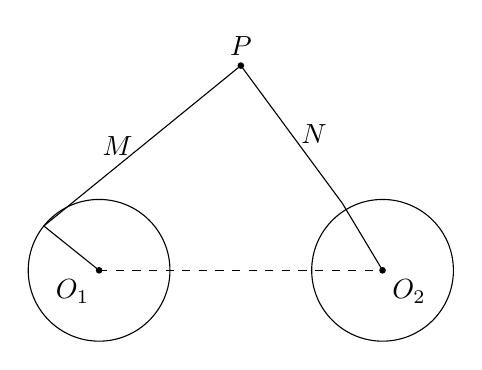
\begin{tikzpicture}[scale=1.0]
  \draw (0,0) circle (0.9);
  \draw (3.6,0) circle (0.9);
  \fill (0,0) circle (1.2pt) node[below left] {$O_1$};
  \fill (3.6,0) circle (1.2pt) node[below right] {$O_2$};
  \draw[dashed] (0,0) -- (3.6,0);
  \coordinate (P) at (1.8,2.6);
  \coordinate (M) at (-0.702,0.563);
  \coordinate (N) at (3.09,0.85);
  \draw (P) -- (M) node[midway, left] {$M$};
  \draw (P) -- (N) node[midway, right] {$N$};
  \fill (P) circle (1.2pt) node[above] {$P$};
  \draw (M) -- (0,0);
  \draw (N) -- (3.6,0);
\end{tikzpicture}
\end{center}
\nopagebreak[4]
\Needspace{4\baselineskip}
\textbf{解析}

\Needspace{5\baselineskip}
以 $O_1O_2$ 所在直线为 $x$ 轴、$O_1O_2$ 中点为原点，则 $O_1(-2, 0)$，$O_2(2, 0)$。设 $P(x, y)$，由切线长公式 $PM^2 = PO_1^2 - 1$，$PN^2 = PO_2^2 - 1$，代入 $PM^2 = 2PN^2$ 得
\nopagebreak[4]
\[
(x+2)^2 + y^2 - 1 = 2\left[(x-2)^2 + y^2 - 1\right],
\]
化简得 $x^2 + y^2 - 12x + 3 = 0$，即 $(x - 6)^2 + y^2 = 33$。

\gkanswer{答案：以 $O_1O_2$ 所在直线为 $x$ 轴、$O_1O_2$ 的中点为原点，轨迹方程为 $(x - 6)^2 + y^2 = 33$。}

\end{answer}
\begin{answer}
\gksolhead{20}{}

\textbf{题目}：

甲、乙两人各射击一次，击中目标的概率分别是 $\dfrac{2}{3}$ 和 $\dfrac{3}{4}$．假设两人射击是否击中目标，相互之间没有影响；每次射击是否击中目标，相互之间没有影响．

(1) 求甲射击 $4$ 次，至少 $1$ 次未击中目标的概率；

(2) 求两人各射击 $4$ 次，甲恰好击中目标 $2$ 次且乙恰好击中目标 $3$ 次的概率；

(3) 假设某人连续 $2$ 次未击中目标，则停止射击．问：乙恰好射击 $5$ 次后，被中止射击的概率是多少？

\Needspace{4\baselineskip}
\textbf{解析}

\gksubpart{(1)}

甲每次未击中的概率为 $\dfrac{1}{3}$，$4$ 次全中的概率为 $\left(\dfrac{2}{3}\right)^4 = \dfrac{16}{81}$，故至少 $1$ 次未击中的概率为 $1 - \dfrac{16}{81} = \dfrac{65}{81}$。

\gksubpart{(2)}

甲恰中 $2$ 次：$\mathrm{C}_4^2\left(\dfrac{2}{3}\right)^2\left(\dfrac{1}{3}\right)^2 = \dfrac{24}{81}$；乙恰中 $3$ 次：$\mathrm{C}_4^3\left(\dfrac{3}{4}\right)^3\left(\dfrac{1}{4}\right) = \dfrac{108}{256}$。相互独立，故概率为 $\dfrac{24}{81}\cdot\dfrac{108}{256} = \dfrac{1}{8}$。

\gksubpart{(3)}

\Needspace{5\baselineskip}
乙恰好射击 $5$ 次后被中止，等价于第 $4$、$5$ 次均未击中，且第 $3$ 次击中，前两次不同时未击中。概率为
\nopagebreak[4]
\[
\left(\frac{1}{4}\right)^2\cdot\frac{3}{4}\cdot\left(1 - \frac{1}{16}\right) = \frac{3}{64}\cdot\frac{15}{16} = \frac{45}{1024}.
\]

\gkanswer{答案（1）：$\dfrac{65}{81}$。}

\gkanswer{答案（2）：$\dfrac{1}{8}$。}

\gkanswer{答案（3）：$\dfrac{45}{1024}$。}

\end{answer}
\begin{answer}
\gksolhead{21}{}

\textbf{题目}：

如图，在五棱锥 $S - ABCDE$ 中，$SA \perp$ 底面 $ABCDE$，$SA = AB = AE = 2$，$BC = DE = \sqrt{3}$，$\angle BAE = \angle BCD = \angle CDE = 120^\circ$．

(1) 求异面直线 $CD$ 与 $SB$ 所成的角（用反三角函数值表示）；

(2) 证明：$BC \perp$ 平面 $SAB$；

(3) 用反三角函数值表示二面角 $B - SC - D$ 的大小（本小问不必写出解答过程）．
\nopagebreak[4]
\begin{center}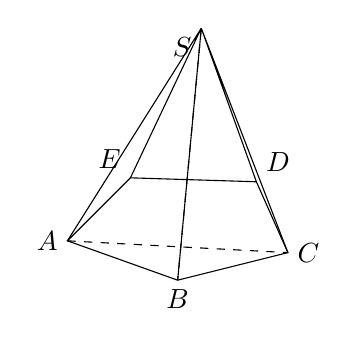
\begin{tikzpicture}[scale=1.0]
  \coordinate (S) at (0.4,2.5);
  \coordinate (A) at (-1.3,-0.2);
  \coordinate (B) at (0.1,-0.7);
  \coordinate (C) at (1.5,-0.35);
  \coordinate (D) at (1.1,0.55);
  \coordinate (E) at (-0.5,0.6);
  \draw (S) -- (A) (S) -- (B) (S) -- (C) (S) -- (D) (S) -- (E);
  \draw (A) -- (B) -- (C) -- (D) -- (E) -- cycle;
  \draw[dashed] (S) -- (B);
  \draw[dashed] (A) -- (C);
  \node[below left] at (S) {$S$};
  \node[left] at (A) {$A$};
  \node[below] at (B) {$B$};
  \node[right] at (C) {$C$};
  \node[above right] at (D) {$D$};
  \node[above left] at (E) {$E$};
\end{tikzpicture}
\end{center}
\nopagebreak[4]
\Needspace{4\baselineskip}
\textbf{解析}

以 $A$ 为原点，$AB$ 所在直线为 $x$ 轴，底面内垂直 $AB$ 的方向为 $y$ 轴，$AS$ 为 $z$ 轴建立空间直角坐标系，则 $A(0,0,0)$，$B(\sqrt{2}, 0, 0)$，$S(0, 0, \sqrt{2})$，$E\left(-\dfrac{\sqrt{2}}{2}, \dfrac{\sqrt{6}}{2}, 0\right)$。

设 $\vec{BC}$ 方向角为 $\varphi$，$\vec{CD}$ 长度为 $d$。由 $\angle BCD = \angle CDE = 120^\circ$ 知 $\vec{CD}$、$\vec{DE}$ 的方向角依次为 $\varphi + 60^\circ$、$\varphi + 120^\circ$，而 $\vec{BE} = \vec{BC} + \vec{CD} + \vec{DE}$ 且 $\left|\vec{BE}\right| = \sqrt{6}$、方向角 $150^\circ$。比较两个方向的合成即得 $\varphi = 90^\circ$、$d = \sqrt{6} - \sqrt{3}$，故 $C(\sqrt{2}, \sqrt{3}, 0)$。

\gksubpart{(1)}

\Needspace{5\baselineskip}
$\vec{CD} = d\left(\cos 150^\circ, \sin 150^\circ, 0\right) \parallel \left(-\sqrt{3}, 1, 0\right)$，$\vec{SB} = \left(\sqrt{2}, 0, -\sqrt{2}\right) \parallel \left(1, 0, -1\right)$。于是
\nopagebreak[4]
\[
\cos\theta = \frac{\left|-\sqrt{3}\right|}{\sqrt{4}\cdot\sqrt{2}} = \frac{\sqrt{6}}{4},
\]
异面直线 $CD$ 与 $SB$ 所成角为 $\arccos\dfrac{\sqrt{6}}{4}$。

\gksubpart{(2)}

由 $\vec{BC} = (0, \sqrt{3}, 0)$ 得 $BC \perp AB$；又 $SA \perp$ 底面故 $BC \perp SA$，而 $AB \cap SA = A$，故 $BC \perp$ 平面 $SAB$。

\gksubpart{(3)}

\Needspace{5\baselineskip}
平面 $SBC$ 的法向量 $\vec{n}_1 = \vec{SB}\times\vec{SC} = \left(\sqrt{6}, 0, \sqrt{6}\right)$；平面 $SCD$ 的法向量 $\vec{n}_2 = \vec{SC}\times\vec{CD} = \left(\sqrt{2}, \sqrt{6}, 3 + \sqrt{2}\right)$。取与 $\vec{SB}$、$\vec{SD}$ 同侧的半平面计算得二面角为钝角，其余弦值为
\nopagebreak[4]
\[
-\frac{14 + 9\sqrt{2}}{34},
\]
故二面角 $B - SC - D$ 的大小为 $\arccos\left(-\dfrac{14 + 9\sqrt{2}}{34}\right)$。

\gkanswer{答案（1）：$\arccos\dfrac{\sqrt{6}}{4}$。}

\gkanswer{答案（2）：由 $BC \perp AB$ 及 $SA \perp$ 底面得 $BC \perp SA$，故 $BC \perp$ 平面 $SAB$。}

\gkanswer{答案（3）：$\arccos\left(-\dfrac{14 + 9\sqrt{2}}{34}\right)$。}

\end{answer}
\begin{answer}
\gksolhead{22}{}

\textbf{题目}：

已知 $a \in \mathbf{R}$，函数 $f(x) = x^2|x - a|$．

(1) 当 $a = 2$ 时，求使 $f(x) = x$ 成立的 $x$ 的集合；

(2) 求函数 $y = f(x)$ 在区间 $[1, 2]$ 上的最小值．

\Needspace{4\baselineskip}
\textbf{解析}

\gksubpart{(1)}

$a = 2$ 时 $f(x) = x^2|x - 2|$。若 $x \geqslant 2$，方程化为 $x^2(x-2) = x$，即 $x\left(x^2 - 2x - 1\right) = 0$，取 $x = 1 + \sqrt{2}$；若 $x < 2$，化为 $x\left(2x - x^2 - 1\right) = 0$，即 $-x(x-1)^2 = 0$，得 $x = 0$ 或 $x = 1$。故解集为 $\{0, 1, 1+\sqrt{2}\}$。

\gksubpart{(2)}

若 $a \leqslant 1$，则在 $[1, 2]$ 上 $|x - a| = x - a$，$f(x) = x^3 - ax^2$，$f'(x) = x(3x - 2a) \geqslant 0$，$f$ 递增，故最小值为 $f(1) = 1 - a$。

若 $1 < a < 2$，则 $a \in [1, 2]$，而 $f(a) = 0$ 且 $f(x) \geqslant 0$，故最小值为 $0$。

若 $a \geqslant 2$，则在 $[1, 2]$ 上 $|x - a| = a - x$，$f(x) = ax^2 - x^3$，$f'(x) = x(2a - 3x)$：$f$ 在 $\left[1, \min\left(2, \dfrac{2a}{3}\right)\right]$ 上递增、之后递减，故最小值在端点取得。$f(1) = a - 1$，$f(2) = 4a - 8$，由 $4a - 8 \leqslant a - 1$ 得 $a \leqslant \dfrac{7}{3}$。故 $2 \leqslant a \leqslant \dfrac{7}{3}$ 时最小值为 $4a - 8$，$a > \dfrac{7}{3}$ 时最小值为 $a - 1$。

\gkanswer{答案（1）：$\{0, 1, 1 + \sqrt{2}\}$。}

\gkanswer{答案（2）：$a\le 1$ 时最小值为 $1-a$；$1<a<2$ 时最小值为 $0$（此时 $x=a\in[1,2]$ 且 $f(a)=0$）；$2\le a\le\dfrac73$ 时最小值为 $4a-8$；$a>\dfrac73$ 时最小值为 $a-1$。}

\end{answer}
\begin{answer}
\gksolhead{23}{}

\textbf{题目}：

\Needspace{5\baselineskip}
设数列 $\{a_n\}$ 的前 $n$ 项和为 $S_n$，已知 $a_1 = 1$，$a_2 = 6$，$a_3 = 11$，且
\nopagebreak[4]
\[
(5n - 8)S_{n+1} - (5n + 2)S_n = An + B,\quad n = 1, 2, 3, \cdots,
\]
其中 $A$，$B$ 为常数．

(1) 求 $A$ 与 $B$ 的值；

(2) 证明数列 $\{a_n\}$ 为等差数列；

(3) 证明不等式 $\sqrt{5a_{mn}} - \sqrt{a_m a_n} > 1$ 对任何正整数 $m$、$n$ 都成立．

\Needspace{4\baselineskip}
\textbf{解析}

\gksubpart{(1)}

$S_1 = 1$，$S_2 = 7$，$S_3 = 18$。代入 $n = 1$：$-3S_2 - 7S_1 = A + B$，即 $A + B = -28$；代入 $n = 2$：$2S_3 - 12S_2 = 2A + B$，即 $2A + B = -48$。解得 $A = -20$，$B = -8$。

\gksubpart{(2)}

\Needspace{5\baselineskip}
先验证 $a_n = 5n - 4$ 满足递推式：此时 $S_n = \dfrac{5n^2 - 3n}{2}$，代入得
\nopagebreak[4]
\[
(5n-8)\cdot\frac{5n^2+7n+2}{2} - (5n+2)\cdot\frac{5n^2-3n}{2} = \frac{-40n - 16}{2} = -20n - 8.
\]
再证唯一性：$n \geqslant 1$ 时 $5n - 8 \neq 0$，故 $S_{n+1}$ 由 $S_n$ 唯一确定；对 $n$ 归纳，若 $a_k = 5k - 4\ (k \leqslant n)$，则 $S_{n+1} = \dfrac{(5n+2)S_n - 20n - 8}{5n-8} = \dfrac{5(n+1)^2 - 3(n+1)}{2}$，从而 $a_{n+1} = S_{n+1} - S_n = 5n + 1 = 5(n+1) - 4$。故 $\{a_n\}$ 为等差数列。

\gksubpart{(3)}

\Needspace{5\baselineskip}
由 (2) 知 $a_m a_n = (5m-4)(5n-4)$，$5a_{mn} = 25mn - 20$。记 $A = 25mn - 20$、$B = (5m-4)(5n-4)$，则 $A - B = 20m + 20n - 36$。由 $\sqrt{A} - \sqrt{B} = \dfrac{A - B}{\sqrt{A} + \sqrt{B}}$ 及 $\sqrt{A} \leqslant 5\sqrt{mn} \leqslant \dfrac{5(m+n)}{2}$、$\sqrt{B} \leqslant 5\sqrt{mn} \leqslant \dfrac{5(m+n)}{2}$ 得
\nopagebreak[4]
\[
\sqrt{5a_{mn}} - \sqrt{a_m a_n} \geqslant \frac{20(m+n) - 36}{5(m+n)}.
\]
当 $m + n \geqslant 3$ 时右端 $\geqslant \dfrac{60 - 36}{5(m+n)}$ 需再细算：由 $m + n \geqslant 3$ 直接得 $20(m+n) - 36 > 5(m+n)$，故不等式成立。当 $m = n = 1$ 时左端为 $\sqrt{5} - 1 > 1$。综上对一切正整数 $m$、$n$ 成立。

\gkanswer{答案（1）：$A = -20$，$B = -8$。}

\gkanswer{答案（2）：$a_n = 5n - 4$，即 $\{a_n\}$ 是首项 $1$、公差 $5$ 的等差数列。}

\gkanswer{答案（3）：$\sqrt{5a_{mn}} - \sqrt{a_m a_n} > 1$ 对一切正整数 $m$、$n$ 成立。}

\end{answer}